% S-N curves for classified welded details (IIW, steel): stress range against cycles.
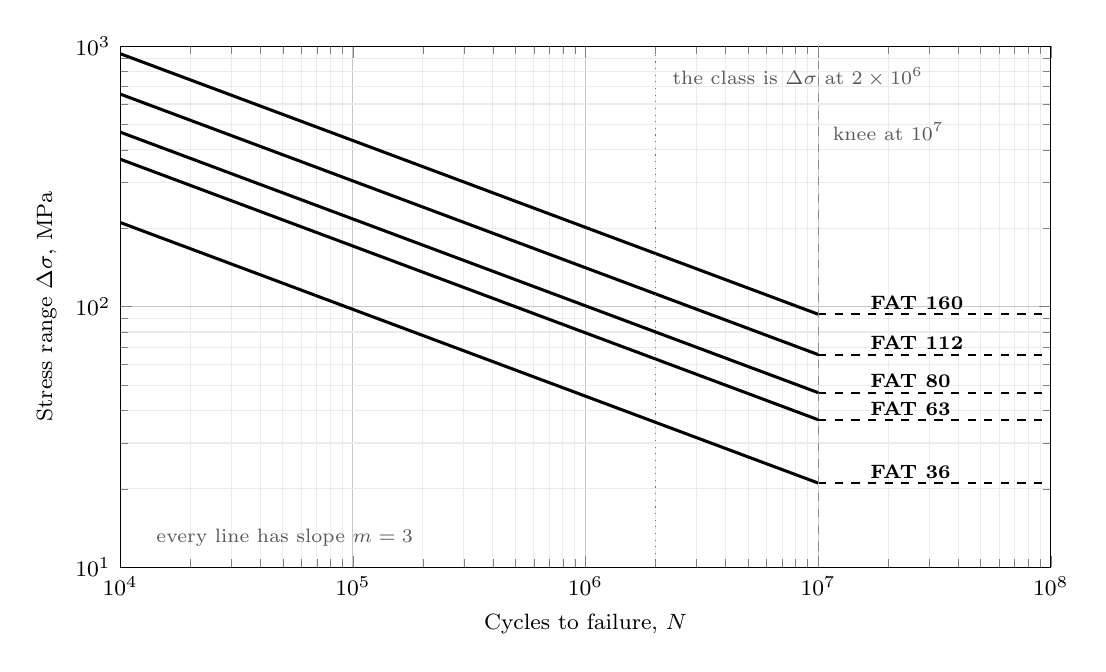
\begin{tikzpicture}
\begin{loglogaxis}[width=13.4cm,height=8.2cm,xmin=1e4,xmax=1e8,ymin=10,ymax=1000,
  xlabel={Cycles to failure, $N$},ylabel={Stress range $\Delta\sigma$, MPa},
  label style={font=\footnotesize},tick label style={font=\footnotesize},grid=both,
  major grid style={black!22},minor grid style={black!8},clip=true]
% FAT lines: N = 2e6 (FAT/ds)^3 down to the knee at 1e7, then flat
\addplot[black,line width=1.1pt,domain=1e4:1e7,samples=2] {160*(2e6/x)^(1/3)};
\addplot[black,line width=0.7pt,dashed,domain=1e7:1e8,samples=2] {93.57};
\addplot[black,line width=1.1pt,domain=1e4:1e7,samples=2] {112*(2e6/x)^(1/3)};
\addplot[black,line width=0.7pt,dashed,domain=1e7:1e8,samples=2] {65.50};
\addplot[black,line width=1.1pt,domain=1e4:1e7,samples=2] {80*(2e6/x)^(1/3)};
\addplot[black,line width=0.7pt,dashed,domain=1e7:1e8,samples=2] {46.78};
\addplot[black,line width=1.1pt,domain=1e4:1e7,samples=2] {63*(2e6/x)^(1/3)};
\addplot[black,line width=0.7pt,dashed,domain=1e7:1e8,samples=2] {36.84};
\addplot[black,line width=1.1pt,domain=1e4:1e7,samples=2] {36*(2e6/x)^(1/3)};
\addplot[black,line width=0.7pt,dashed,domain=1e7:1e8,samples=2] {21.05};
\addplot[black!55,line width=0.4pt,dotted] coordinates {(2e6,10) (2e6,1000)};
\node[font=\scriptsize,anchor=south west,text=black!65] at (axis cs:2.15e6,640) {the class is $\Delta\sigma$ at $2\times10^{6}$};
\node[font=\scriptsize\bfseries,anchor=south west,inner sep=1.5pt] at (axis cs:1.6e7,93.6) {FAT 160};
\node[font=\scriptsize\bfseries,anchor=south west,inner sep=1.5pt] at (axis cs:1.6e7,65.5) {FAT 112};
\node[font=\scriptsize\bfseries,anchor=south west,inner sep=1.5pt] at (axis cs:1.6e7,46.8) {FAT 80};
\node[font=\scriptsize\bfseries,anchor=south west,inner sep=1.5pt] at (axis cs:1.6e7,36.8) {FAT 63};
\node[font=\scriptsize\bfseries,anchor=south west,inner sep=1.5pt] at (axis cs:1.6e7,21.05) {FAT 36};
\node[font=\scriptsize,anchor=south west,text=black!65] at (axis cs:1.05e7,400) {knee at $10^{7}$};
\draw[black!45,line width=0.3pt,dashed] (axis cs:1e7,10) -- (axis cs:1e7,1000);
\node[font=\scriptsize,anchor=south west,text=black!65] at (axis cs:1.3e4,11) {every line has slope $m=3$};
\end{loglogaxis}
\end{tikzpicture}
